%\begin{frame}
%    \frametitle{\insertsection}
%    \framesubtitle{\insertsubsection}
%
%    \begin{itemize}
%        \item<1-> Strategien zur Resilienzsteigerung in verteilten Systemen
%        \item<2-> Fehlertoleranz und Ausfallsicherheit
%        \item<3-> Praktische Implementierungen wie Circuit Breaker, Retry-Muster
%        \item<4-> Ziel: Absicherung moderner Anwendungen gegen Störungen
%    \end{itemize}
%\end{frame}

\section{Resilienz und Fehlertoleranz}
\subsection{Begriffsklärung}

\begin{frame}
    \frametitle{\insertsection}
    \framesubtitle{\insertsubsection}

    \begin{block}{Motivation}
        \begin{itemize}

        \end{itemize}
    \end{block}
\end{frame}
%...

\subsection{Motivation}

\begin{frame}
    \frametitle{\insertsection}
    \framesubtitle{\insertsubsection}

    \begin{block}{Motivation}
        \begin{itemize}
            \item Schutz vor Ausfällen in geschäftskritischen Anwendungen
            \item Reduktion betrieblicher Kosten und Steigerung der Nutzerzufriedenheit
            \item Anforderungen an Verfügbarkeit in regulierten Branchen
        \end{itemize}
    \end{block}
\end{frame}

\begin{frame}
    \frametitle{\insertsection}
    \framesubtitle{\insertsubsection}

    \begin{itemize}
        \item Verbreitung von Microservices und Cloud-Technologien
        \item Herausforderungen durch Kommunikationsausfälle und Spitzenlasten
        \item Bedarf an innovativen Resilienzmustern
    \end{itemize}
\end{frame}

\section{Strategien}
\subsection{Resilienzstrategien}
\begin{frame}
    \frametitle{\insertsection}
    \framesubtitle{\insertsubsection}

    \begin{itemize}
        \item Redundanz
        \item Partitionierung
        \item Skalierung
    \end{itemize}
\end{frame}

\subsection{Fehlertoleranzstrategien}

\begin{frame}
    \frametitle{\insertsection}
    \framesubtitle{\insertsubsection}

    \begin{itemize}
        \item Fehlerbehandlung und -isolierung
        \item Nutzung von Fallback-Mechanismen
        \item Vermeidung kaskadierender Fehler
    \end{itemize}
\end{frame}

\section{Pattern und Konzepte}
\subsection{Circuit-Breaker}

\begin{frame}
    \frametitle{\insertsection}
    \framesubtitle{\insertsubsection}

    \begin{itemize}
        \item Isoliert fehlerhaftxe Dienste
        \item Unterbricht Anfragen bei wiederholtem Fehler.
        \item Verhindert kaskadierende Ausfälle
    \end{itemize}
\end{frame}

\subsection{Circuit-Breaker: Zustandsdiagramm}
\begin{frame}
    \frametitle{\insertsection}
    \framesubtitle{\insertsubsection}

    \begin{figure}
        \pgfdeclarelayer{background}
        \pgfdeclarelayer{foreground}
        \pgfsetlayers{background,main,foreground}
    % Define a few styles and constants
        \tikzstyle{state} = [draw, rounded corners,
        text centered, minimum height=3em, minimum width=4em]
        \centering
        \centering
        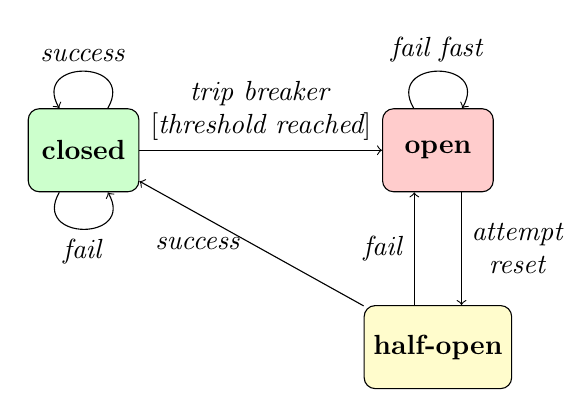
\begin{tikzpicture}[
    %scale=0.6, every node/.style={scale=0.6}
        ]
            \node (closed) [state, fill=green!20] {\textbf{closed}};
            \node (open) [state, fill=red!20, right of=closed, node distance =4.5cm] {\textbf{open}};
            \node (halfopen) [state, fill=yellow!20, below of=open, node distance =2.5cm] {\textbf{half-open}};
            \draw [->] (closed) -- (open) node[above,midway,align=center] {\textit{trip breaker}\\\textit{$[$threshold
            reached$]$}};
            \draw [->] (halfopen) -- (closed) node[left,midway] {\textit{success}};
            \draw [transform canvas={xshift=-0.3cm},->] (halfopen) -- (open) node[left,midway] {\textit{fail}};
            \draw [transform canvas={xshift=0.3cm},->] (open) -- (halfopen) node[right,midway,align=center]
                {\textit{attempt}\\\textit{reset}};
            \path[]	(open)   edge[loop, in=60,out=120, looseness=3,->] node[above]  {\textit{fail fast}} (open);
            \path[]	(closed)   edge[loop, in=60,out=120, looseness=3,<-] node[above]  {\textit{success}} (closed);
            \path[]	(closed)   edge[loop, in=240,out=300, looseness=3,<-] node[below]  {\textit{fail}} (closed);
        \end{tikzpicture}
        \caption{Circuit Breaker Zustandsdiagramm} % TODO Quelle
        \label{cb-fsm}
    \end{figure}
\end{frame}

\subsection{Circuit-Breaker: Vorteile}
\begin{frame}
    \frametitle{\insertsection}
    \framesubtitle{\insertsubsection}

    \begin{itemize}
        \item Verhindert kaskadierende Ausfälle in verteilten Systemen.
        \item Verbesserte Systemstabilität durch Isolierung fehlerhafter Dienste.
        \item Bessere Benutzererfahrung durch Fallback-Mechanismen.
        \item Unterstützt Resilienz und Wiederherstellung in kritischen Systemen.
    \end{itemize}
\end{frame}

\subsection{Circuit-Breaker: Nachteile}
\begin{frame}
    \frametitle{\insertsection}
    \framesubtitle{\insertsubsection}

    \begin{itemize}
        \item Erhöhte Komplexität in der Implementierung und Wartung.
        \item Risiko von Fehlkonfiguration (z. B. falsche Schwellenwerte).
        \item Zusätzlicher Overhead durch Überwachung und Statusverwaltung.
        \item Fallback-Daten können veraltet oder ungenau sein.
    \end{itemize}
\end{frame}

\subsection{Retry-Muster}
\begin{frame}
    \frametitle{\insertsection}
    \framesubtitle{\insertsubsection}

    \begin{itemize}
        \item Automatisches Wiederholen fehlgeschlagener Operationen
        \item Nutzung von Exponential Backoff
        \item Verbesserung der Resilienz bei temporären Fehlern
    \end{itemize}
\end{frame}

\subsection{Retry-Muster: Sequenzdiagramm}
\begin{frame}
    \frametitle{\insertsection}
    \framesubtitle{\insertsubsection}

    \begin{figure}[h]
        \centering
        \includegraphics[height=0.5\textheight]{images/retry-pattern}
        \caption{Sequenzdiagramm des Retry Patterns}
    \end{figure}
\end{frame}

\subsection{Retry-Muster: Vorteile}
\begin{frame}
    \frametitle{\insertsection}
    \framesubtitle{\insertsubsection}

    \begin{itemize}
    \item Reduziert die Wahrscheinlichkeit eines vollständigen Anwendungsabsturzes bei vorübergehenden Fehlern.
    \item Verbessert die Zuverlässigkeit, indem kurzfristige Probleme (z. B. Netzwerkprobleme) automatisch überwunden werden.
    \item Ermöglicht ein einheitliches Fehlerbehandlungsmodell in einer Anwendung.
\end{itemize}
\end{frame}

\subsection{Retry-Muster: Nachteile}
\begin{frame}
    \frametitle{\insertsection}
    \framesubtitle{\insertsubsection}

    \begin{itemize}
        \item Erhöhte Komplexität in der Implementierung und Wartung.
        \item Verzögert die Gesamtverarbeitung, wenn ein Vorgang wiederholt fehlschlägt.
        \item Kann echte, dauerhafte Fehler verschleiern, wenn nur wiederholt wird, ohne die Ursache zu analysieren.
        \item Nicht jeder Fehler ist vorübergehend (z. B. Authentifizierungsfehler), was zu unnötigen Wiederholungen führt.
    \end{itemize}
\end{frame}

\subsection{Kombination mit Circuit-Breaker}

\begin{frame}
    \frametitle{\insertsection}
    \framesubtitle{\insertsubsection}

    \begin{itemize}
        \item Stoppt Wiederholungen bei permanenten Fehlern
        \item Ermöglicht Systemen, sich zu erholen
        \item Optimiert Ressourcennutzung
    \end{itemize}
\end{frame}

\subsection{Load Balancing}

\begin{frame}
    \frametitle{\insertsection}
    \framesubtitle{\insertsubsection}

    \begin{itemize}
        \item Verteilung der Last auf mehrere Server
        \item Strategien: Round Robin, Least Connection, Resource Based
        \item Verbesserung von Leistung und Ausfallsicherheit
    \end{itemize}
\end{frame}

\subsection{Load Balancer: Architekturdiagramm}
\begin{frame}
    \frametitle{\insertsection}
    \framesubtitle{\insertsubsection}

    \begin{figure}[h]
        \centering
        \includegraphics[height=0.5\textheight]{images/loadbalancer}
        \caption{Architekturdiagramm mit einem zentalen Load Balancer}
    \end{figure}
\end{frame}

\subsection{Health Checks bei Load Balancing}
\begin{frame}
    \frametitle{\insertsection}
    \framesubtitle{\insertsubsection}

    \begin{itemize}
        \item Überwachung der Zustände von Diensten
        \item Vermeidung von Überlastungen
        \item Umgang mit fehlerhaften Knoten
    \end{itemize}
\end{frame}

\section{Fazit}
\subsection{Was wurde gemacht?}

\begin{frame}
    \frametitle{\insertsection}
    \framesubtitle{\insertsubsection}

    \begin{itemize}
        \item Analyse und Implementierung von Resilienzstrategien
        \item Fallstudien und Praxisbeispiele
        \item Implementierungen in Python
    \end{itemize}
\end{frame}

\subsection{Fallstudie: Netflix}
\begin{frame}
    \frametitle{\insertsection}
    \framesubtitle{\insertsubsection}

    \begin{itemize}
        \item Nutzung von Hystrix für Circuit-Breaker
        \item Dynamisches Load Balancing
        \item Skalierung und Fehlertoleranz
    \end{itemize}
\end{frame}

%\section{Ausblick}
%
%\begin{frame}
%    \frametitle{\insertsection}
%    \framesubtitle{\insertsubsection}
%
%    \begin{itemize}
%        \item Circuit Breaker und Retry-Muster als effektive Mechanismen
%        \item Kombination verschiedener Strategien verbessert Resilienz
%        \item Bedeutung von agilen Methoden zur kontinuierlichen Verbesserung
%    \end{itemize}
%\end{frame}

\section{Diskussion}

\begin{frame}
    \frametitle{\insertsection}
    \framesubtitle{\insertsubsection}

    \begin{itemize}
        \item Erweiterung der Strategien auf andere Szenarien
        \item Entwicklung neuer Muster zur Resilienzsteigerung
        \item Untersuchung ökonomischer Auswirkungen
    \end{itemize}
\end{frame}

\section{Quellen}

\begin{frame}
    \frametitle{\insertsection}
    \framesubtitle{\insertsubsection}

    \begin{itemize}
        \item
    \end{itemize}
\end{frame}
